\section{Fatigue}
	While dealing with fatigue we have to determine the mean value $\sm$ and the amplitude $\sa$ of the varying stress state on the section, and considering the maximum $\smax$ and minimum $\smin$ equivalent stresses on the section we have
	\begin{equation}
		\sm = \frac{\smax +\smin}{2} \qquad \qquad \qquad \sa = \frac{\smax-\smin}{2}
	\end{equation} 
	
	It's also necessary to compute the \textbf{notch fatigue factor} $K_f$ depending on the stress concentration factor $K_t$ (page \pageref{fig:stressconcentrationfactors}) of the particular critical section and the \textbf{notch sensitivity} $q$ that can be assessed by looking at some diagrams (figure \ref{fig:notchsens}, if cannot be determined, $q=1$ is the conservative choice). With that we have
	\begin{equation} \label{eq:notchfactor}
		K_f = 1 + q(K_t-1)
	\end{equation}
	
	\begin{figure}[bht]
		\centering 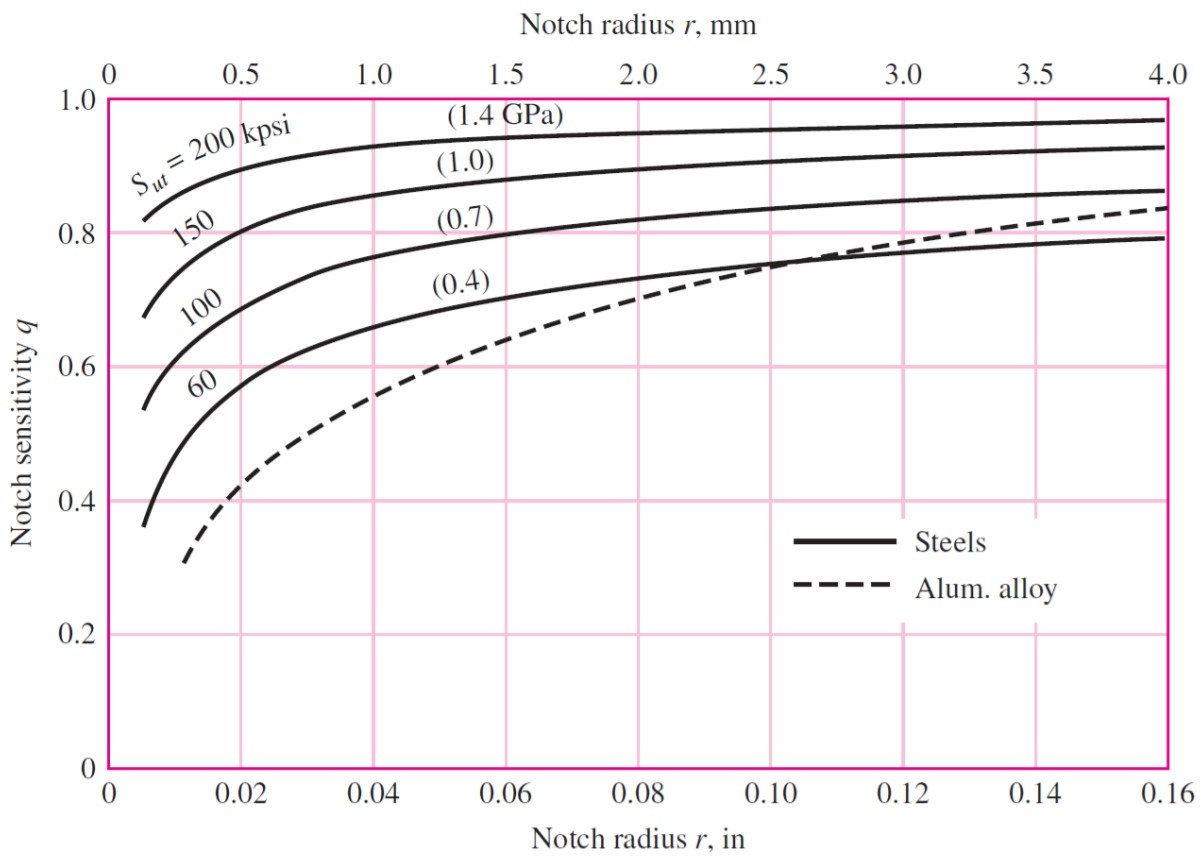
\includegraphics[width=11cm]{notch-factor}
		\caption{notch sensitivity factor $q$ for different steels and aluminium.} \label{fig:notchsens}
	\end{figure}
	
	To relate the laboratory samples with real-production pieces we have to compute the \textbf{allowable} stress $\sall$ depending on the coefficients $C_s,C_d,C_l$ and the safety factor $\phi$:
	\begin{equation}
		\sall = \frac{C_s C_d C_l}{\phi} \sigma_{lim}
	\end{equation}
	In particular
	\begin{itemize}
		\item $C_s$ is the \textbf{surface} finish factor computed using equation \begin{equation} \label{eq:surfacefinish}
			C_s = a \,\sigma_r ^b
		\end{equation}
		where $\sigma_r$ is the ultimate tensile strength (UTS) of the material measured in $MPa$; the coefficient $a$ and the exponent $b$ can be determined by table \ref{tab:surfacefinish} depending on the surface finish;
		
		\begin{table}[bt]
			\centering
			\rule{0.8\linewidth}{1pt}
			\caption{coefficients to determine the surface effect coefficient (equation \ref{eq:surfacefinish}).}
			\label{tab:surfacefinish}
			\begin{tabular}{r | c  c}
				\textbf{surface finish} & coefficient $a$ & exponent $b$ \\ \hline
				ground & 1.58 & -0.085 \\
				machined or cold-drawn & 4.51 & -0.265 \\
				hot-rolled & 57.7 & -0.718 \\
				as-forged & 272 & -0.995
			\end{tabular}
			\rule{0.8\linewidth}{1pt}
		\end{table}
		
		
		\item $C_d$ is the \textbf{dimension} coefficient that depends on the equivalent diameter $d_{eq}$ (usually calculated as $\sqrt \frac 4 \pi A$) following the system\begin{equation} \label{eq:dimensioncoefficient}
			C_d = \begin{cases}
				1 & d_{eq} < 8mm \\
				1.189 d_{eq} ^{-0.097} \quad & 8mm < d_{eq}  < 250mm \\
				0.6 & d_{eq}  > 250mm
			\end{cases}
		\end{equation}
	
		\item $C_l$ is the \textbf{load} coefficient depending on the nature of the oscillation of the stress state, in particular
		\begin{equation}
			C_{l} = \begin{cases}
				1 & \textrm{bending, torsion} \\
				0.6 \quad & \textrm{axial loading}
			\end{cases}
		\end{equation}
	\end{itemize}

	Computed so $\sall$, we have to transform the fatigue problem with mean value $\sm$ and amplitude $\sa$ to a laboratory condition where $\sm^* = 0$ (in order to use the SN curves); this can be done by using the iso-critical stress method (figure \ref{fig:isocritical}) that, with a linear relation, allows to compute the equivalent pure amplitude oscillation load of 
	\begin{equation}
		\sa^* = \sigma_y \frac{\sa}{\sigma_y - \sm}
	\end{equation}

	In order to include the possible plasticisation due to the non-zero mean stress, it's possible to use the following criteria that modify the nominal mean stress $\sigma_{m,nom}$ depending from the stress concentration factor $K_t$:
	\begin{equation} \label{eq:plasticization}
		\sigma_m = \begin{cases}
			\sigma_{m,nom} & K_t \sigma_{max} > \sigma_y \\
			K_f\sigma_{m,nom} \quad & K_t \sigma_{max} \leq \sigma_y \\
		\end{cases}
	\end{equation}
	
	\begin{SCfigure}[2][bht]
		\centering 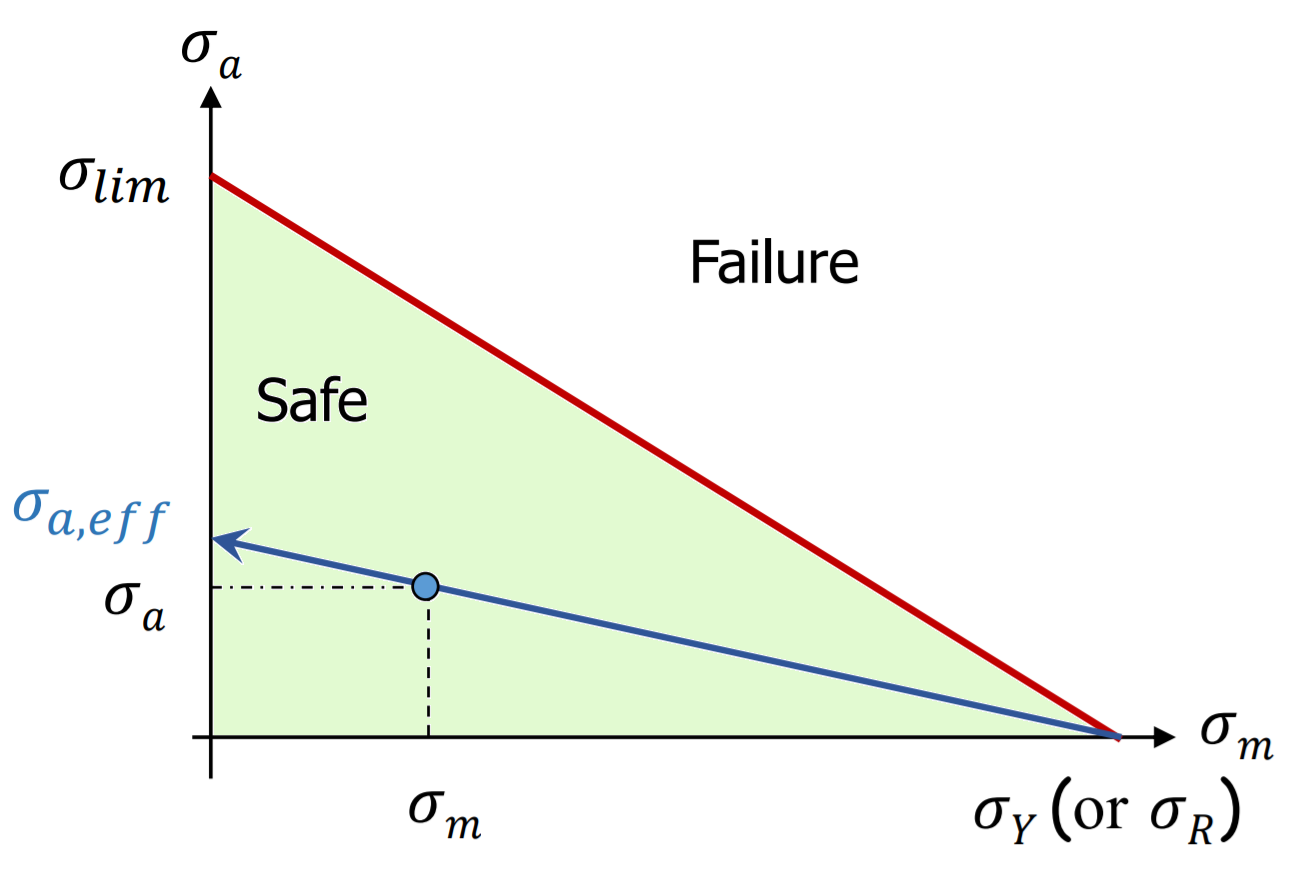
\includegraphics[width=5.5cm]{isocritical-fatigue}
		\caption{scheme used by the iso-critical stress method in order to the determine the equivalent pure amplitude $\sa^*$ oscillation stress of the piece.} \label{fig:isocritical}
	\end{SCfigure}

\subsection{SN diagrams}
	The simplest function that's used to related the number $N_f$ of cycle to failure with the alternate stress $\sa$ is determined by the \textbf{Basquin law} stating
	\begin{equation} \label{eq:basquin}
		\sa = C N_f^{-1/k}
	\end{equation}
	As shown in figure \ref{fig:basquin}, such relation can be easily fitted in a log-log plot. Known the fatigue limit $\sigma_{lim}$ and the related cycles to failure $N_{lim}$ and another experimental point $\sigma_0,N_0$, using the following expression we can determine
	\begin{equation}
		\frac 1 k = \frac{-\log \left( \frac{\sigma_{lim}}{\sigma_0} \right)}{\log\left( \frac{N_{lim}}{N_0} \right)} \qquad \qquad \qquad C = \frac{\sigma_{lim}}{N_{lim}^{-1/k}}
	\end{equation}
	For steels material the fatigue limit can be regarded as
	\[ \sigma_{lim} = \begin{cases}
		0.5 \sigma_r \qquad &\sigma_r \leq 1400 MPa \\ 700 MPa \qquad & \sigma_r > 1400 MPa
	\end{cases} \]
	\begin{SCfigure}[2][bht]
		\centering 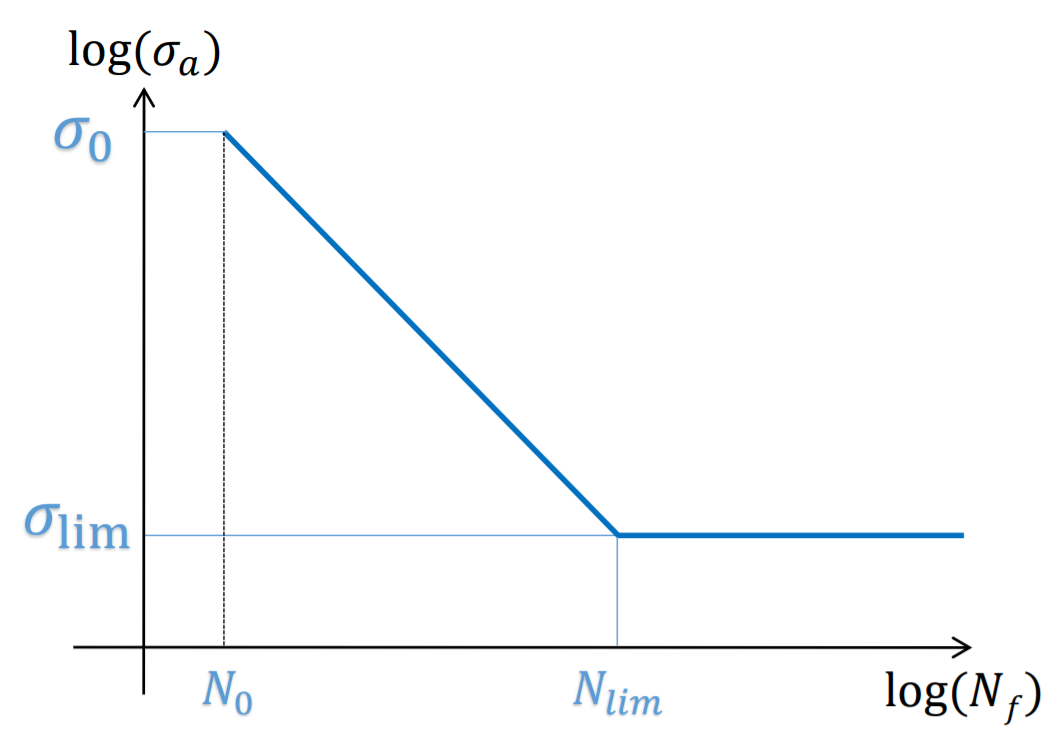
\includegraphics[width=6cm]{SNbasquin}
		\caption{scheme used by the iso-critical stress method in order to the determine the equivalent pure amplitude $\sa^*$ oscillation stress of the piece.} \label{fig:basquin}
	\end{SCfigure}

\subsection{Damage}
	The \textbf{damage} $D$ related to fatigue considering multi-variable loads can be taken into account using a linear operator 
	\begin{equation}
		D = \sum_i \frac{n_i}{N_{f,i}} \leq 1
	\end{equation}
	where $n_i$ is the actual number of cycles at mean stress $\sigma_{m,i}$ and amplitude $\sigma_{a,i}$ that determines a number of cycles to fracture of $N_{f,i}$ (as previously discussed). Using conventional method if $\sigma_a^*$ is less then the limit $\sigma_{lim}$, then the related damage should be zero, however this isn't true. In order to take into account such damage we have to revise the SN diagrams by giving a non-zero slope after the $N_{lim}$ cycles (as shown in figure \ref{fig:damage}) considering the law
	\[ \sa = C' N_f^{-1/(2k-1)} \]
	where the constant $C'$ is computed in order to obtain continuity in the diagram. In this case remember that the actual stress limit of the part is different than the laboratory sample and we have to consider
	\begin{equation}
		\sigma_{lim,part} = \frac{C_sC_dC_l}{K_f}\sigma_{lim}
	\end{equation}
	
	\begin{SCfigure}[2][bht]
		\centering 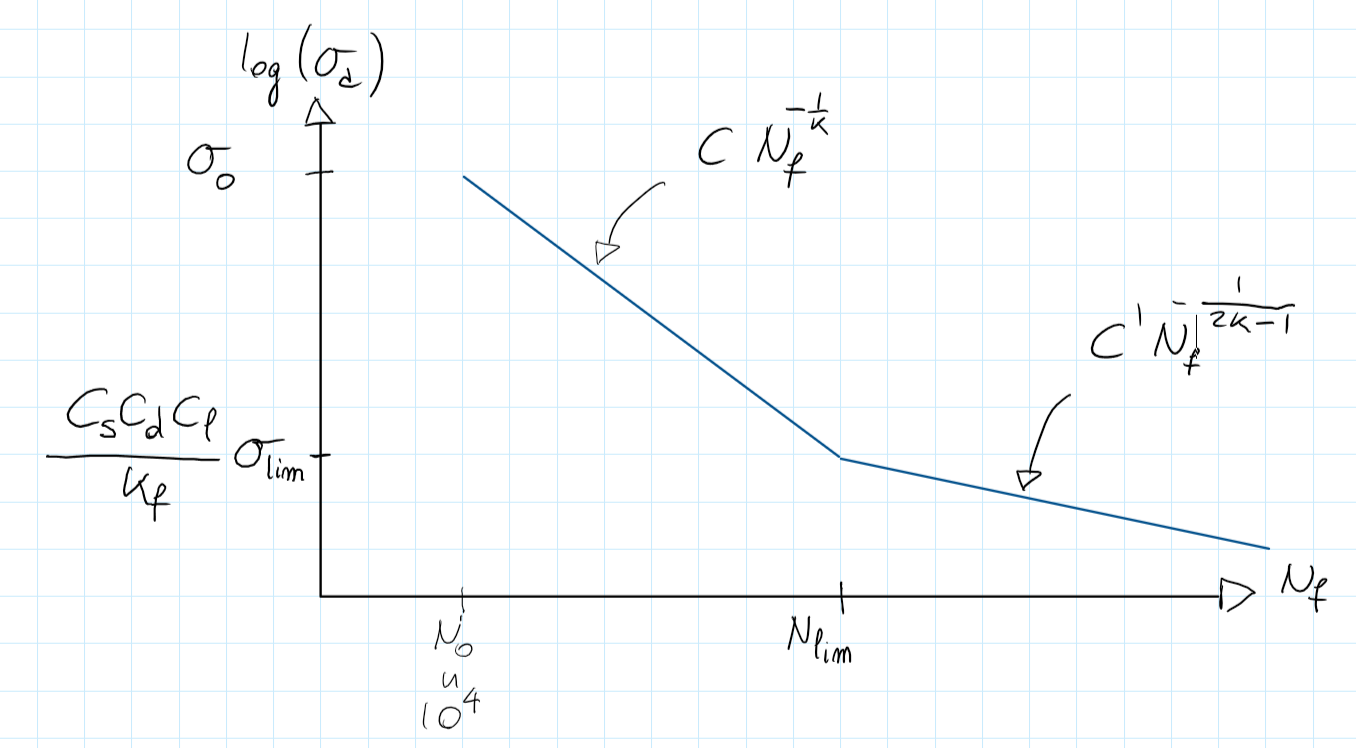
\includegraphics[width=7cm]{SNdamage}
		\caption{revision of the SN diagram that has to be considered while dealing with calculation of the damage in the structure.} \label{fig:damage}
	\end{SCfigure}
	
	
	
	
	
	
	
	
	
	
	
	
	
%	\vspace{5cm}
%
%\begin{multicols} 2
%\subsection*{SN diagrams}
%	The simplest function that's use to relate the number of cycle to failure $N_f$ with the alternate stress $\sigma_a$ is the Basquin law
%	\begin{equation}
%		\sigma_a = C N_f ^{-\frac 1 k}
%	\end{equation}
%	\begin{center}
%		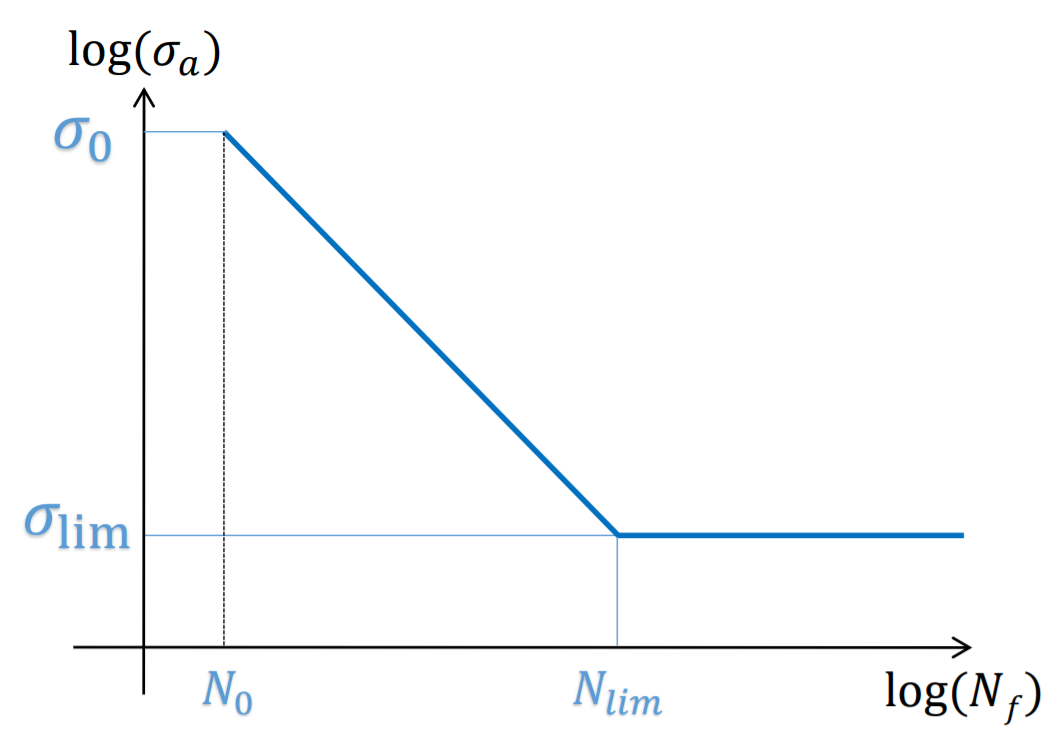
\includegraphics[width=5cm]{SNbasquin}
%	\end{center}
%	
%	This relation is made to fit, as seen in the shown diagram, the linear logarithmic relation between the stress and the cycles to failure; in particular known the limit tension $\sigma_{lim}$ and the related cycle $N_{lim}$ and another experimental point $\sigma_0, N_0$, it's possible to compute the coefficient $C$ and $1/k$ of the law:
%	\[ \frac 1 k = \frac{-\log \left( \frac{\sigma_{lim}}{\sigma_0} \right) }{\log \left( \frac{N_{lim}}{N_0} \right)}  \qquad C = \frac{\sigma_{lim}}{N_{lim}^{-\frac 1 k}} \]
%	In general the fatigue limit (for steels) can be computed as
%	\[ \sigma_{lim} = \begin{cases}
%		0.5 \sigma_r \qquad & \sigma_r \leq 1400MPa \\
%		700 MPa & \sigma_r>1400MPa
%	\end{cases}  \]
%
%\subsection*{Damage}
%	In order to take into account the damage $D$ due to fatigue it's possible to use a linear operation (that allow to take into account multi-variable load) defined as
%	\[ D = \sum_i \frac{n_i}{N_{f,i}} \leq 1 \]
%	where $n_i$ is the number of cycles at certain combination of cyclic stress with mean value $\sigma_{m,i}$ and amplitude $\sigma_{a,i}$ that determines a number of fatigue fracture cycles $N_{f,i}$. By using conventional method to compute $N_f$, if the component is subject to a stress less than $\sigma_{lim}$ than the damage should be zero, but in reality it's not: in this case we revise the SN diagram in order to take into account that factor by using not a straight line after $N_{lim}$, but one relation in the form
%	\[ \sigma_a = C'N_f^{-\frac{1}{2k-1}} \]
%	\begin{center}
%		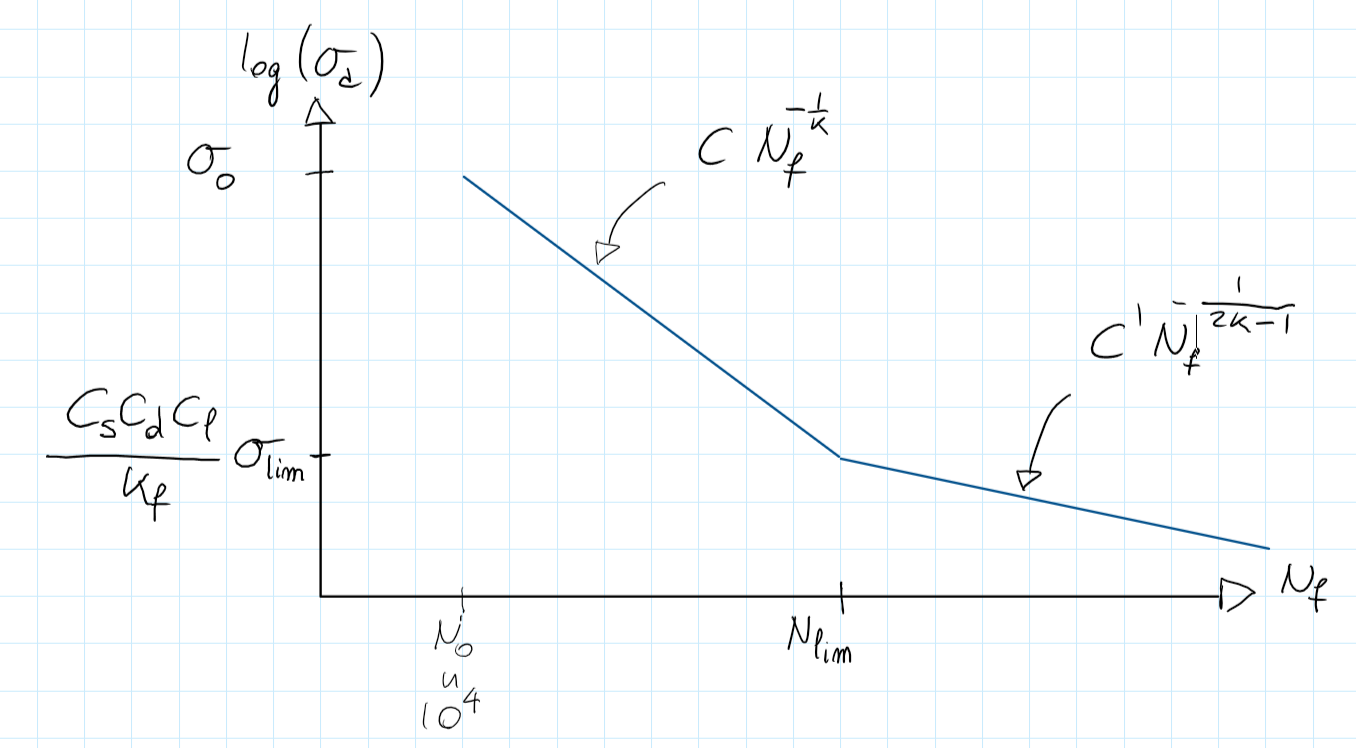
\includegraphics[width=7cm]{SNdamage}
%	\end{center}
%	Pay attention when doing so at including also the effect of the coefficients $C_s,C_d,C_l$ and $K_f$.
%
%
%
%\end{multicols}
%
%
%
%
%
%
